% Copyright 2020 by Robert Hildebrand
%This work is licensed under a
%Creative Commons Attribution-ShareAlike 4.0 International License (CC BY-SA 4.0)
%See http://creativecommons.org/licenses/by-sa/4.0/


%\documentclass[../open-optimization/open-optimization.tex]{subfiles}
%
%\begin{document}

\chapter{Algorithms and Complexity}
\todoChapter{ 60\% complete. Goal 80\% completion date: August 20\\
Notes: }
\label{sec:complexity}
\begin{outcome}
\begin{enumerate}
\item Describe asymptotic growth of functions using Big-O notation.
\item Analyze algorithms for the asymptotic runtime.
\item Classify problem types with respect to notions of how difficult they are to solve.
\end{enumerate}
\end{outcome}




How long will an algorithm take to run?   How difficult might it be to solve a certain problem?   Is the knapsack problem easier to solve than the traveling salesman problem?  Or the matching problem?  
How can we compare the difficulty to solve these problems?

 

We will understand these questions through complexity theory.   We will first use "Big-O" notation to simplify asymptotic analysis of the runtime of algorithms and the size of the input data of an algorithm.  

We will then classify problem types as being either easy ( in the class P) or probably very hard (in the class NP Hard).  We will also learn about the problem classes NP, and NP-Complete.  

To begin, watch these videos (\href{https://www.youtube.com/watch?v=aXXWXz5rF64}{Video 1}, \href{https://youtu.be/TZRWRjq2CAg}{Video 2} )about sorting algorithms.  Notice how a different algorithm can produce a much different number of steps needed to solve the problem.  The first video explains bubble sort and quick sort. The second video explains insertion sort, and then described the analysis of the algorithms (how many comparisons they make as the number of balls to sort grows.    Pay attention to this analysis as this is very crucial in this module.



           

This \href{https://youtu.be/__vX2sjlpXU}{video} is a great introduction to the basic idea of Big-O notation.  We will go over the more formal definition.

    

Here are two great videos about P versus NP (\href{https://youtu.be/EHp4FPyajKQ}{Video 1}, \href{https://youtu.be/YX40hbAHx3s}{Video 2}).  
%
%There is one more complexity class that I find fascinating.  This is called the class of "undecidable problems".   These are problems to which there cannot exist an algorithm general to solve them.  Although this class will not be a focus of this course, if you're interested, watch the following videos that explain the "halting problem", the first problem that was proved to be undecidable. 

         


%\includegraphics[scale = 0.5]{enigma}
%
%\includegraphics[scale = 0.5]{enigma-break}
%
%\url{https://en.wikipedia.org/wiki/Alan_Turing}

\section{Big-O Notation}
We begin with some defintions that relate the rate of growth of functions.   The functions we will look at in the next section will describe the runtime of an algorithm.  



\begin{example}{Relations of functions}{}
We want to understand the asymptotic growth of the following functions:
\begin{itemize}
\item $f(n) = n^2 + 5$,
\item $g(n) = n^3 - 10n^2 -10$.
%\item $h(n) = \tfrac{1}{1000}n^3$
%\item $r(n) = n^4$
\end{itemize}

When we discuss \emph{asymptotic growth}, we don't care so much what happens for small values of $n$, and instead, we want know what happens for large values of $n$.

Notice that 
\begin{equation}
\lim_{n \to \infty} \frac{f(n)}{g(n)} = 0.
\end{equation}
This is because as $n$ gets large, $g(n) >> f(n)$.  However, this does not preclude the possibility that $g(n) < f(n)$ for some small values of $n$, (i.e., $n=1,2,3$).

We can, however see that $g(n) > f(n)$ whenever $n \geq N:= 20$ (it is probably true for a smaller value of $n$, but for the sake of the analysis, we don't care).

Thus, we want to say that $g(n)$ grows faster than $f(n)$.

%\noindent \textbf{$f(n), h(n)$}\\
%Notice that $h(n)$ and $f(n)$ bear the same relation as $g(n)$ and $f(n)$, but this time we must take the value $N$ to be much larger to ensure that $h(n) > f(n)$ for all $n \geq N$.
%
%Again though, we notice that $h(n)$ is function that grows faster.
%
%
%\noindent \textbf{$f(n), h(n)$}\\
%
%
%
%
\end{example}

\begin{example}{Asymptotic Technicality}{}
It may be that we consider functions that are not strictly increasing after some point.  For example,
\begin{itemize}
\item $f(n) = \sin(n)(n^2 + 5)$,
\item $g(n) = 10n^2 -10$.
\end{itemize}

Still, we would like to say that $f(n)$ is bounded somehow by $g(n)$.  But!   The limit $\lim_{n \to \infty} \tfrac{f(n)}{g(n)}$ does not exist!

For this, we use the $\lim\sup$ notation.That is, we notice that 
\begin{equation}
\limsup_{n\to \infty} \tfrac{f(n)}{g(n)} < \infty.
\end{equation}
This completely captures our goal here.  However, we will give an alternative definition that allows us to not have to think about the $\limsup$.
\end{example}


\begin{figure}[h]
\begin{center}
\begin{tikzpicture}
    \draw[->]  (0,0)coordinate(O) -- (8,0) node[anchor=north] {$n$};
    \draw[->]  (0,0) -- (0,5);

\draw[domain=0:8,smooth,variable=\x,blue,name path=c1] plot ({\x},{0.5*\x+2*sin(\x r)+1})node[right]{$c\cdot g(n)$};
\draw[domain=0:8,smooth,variable=\x,blue,name path=c0] plot ({\x},{0.3*0.5*\x+0.3*2*sin(\x r)+0.3*1})node[right]{$g(n)$};
\draw[domain=0:8,smooth,variable=\x,red,name path=c2] plot ({\x},{0.2*\x+0.5*sin(\x r)+2})node[right,black]{$f(n)$};
\fill[red,name intersections={of=c1 and c2}]
    (intersection-1) circle (2pt)
    (intersection-2) circle (2pt)
        (intersection-3) circle (2pt) ;

\draw[dashed] (intersection-3) -- (intersection-3|-O) node[below]{$n_0$};
\end{tikzpicture}
\end{center}
\caption{Example of Big-O notation: $f(n) = O(g(n))$.   We see that for all $n \geq n_0$, we have $c \cdot g(n) \geq f(n)$.  }
\end{figure}



\begin{definition}{Big-O}{}
For two functions $f(n)$ and $g(n)$, we say that $f(n) = O(g(n))$ if there exist positive constants $c$ and $n_0$ such that 
\begin{equation}
\label{eq:bigO}
0 \leq f(n) \leq c\, g(n) \ \ \text{ for all } \ \ \ n \geq n_0.
\end{equation}
\end{definition}



%\includefigurestatic[Example of Big O notation: $f(x) \in O(g(x))$ as there exists $c > 0 $ (e.g. $c = 1$) and $x_0$ (e.g. $x_0 = 5$) such that $f(x) \leq cg(x)$ whenever $x \geq x_0$.]{wiki/File/Big-O-notation.png}


%We can also use Big-O to denote a set as
%\begin{multline}
%O(g(n)) := \{ f(n) :\text{ there exist positive constants $c$ and $n_0$ such that}\\ \text{$0 \leq f(n) \leq c\,g(n)$, for all $n \geq n_0$}\}.
%\end{multline}
\begin{example}
\label{ex:bigO}
Consider $f(n) = 5 n^2 + 10n + 7$ and $g(n) = n^2$.  We want to show that $f(n) = O(g(n))$.  

Let's try $c = 22$ and $n_0 = 1$.  We need to show that \autoref{eq:bigO} is satisfied.

Note first that we always have
\begin{enumerate}
\item $n^2 \leq n^2 \ \ \text{ and therefore } \ \ 5n^2 \leq 5n^2$
\end{enumerate}
Note that if $n \geq 1$, then 
\begin{enumerate}
\setcounter{enumi}{1}
\item $n \leq n^2 \ \ \text{ and therefore } \ \ 10n \leq 10 n^2$
\item $1 \leq n^2 \ \ \text{ and therefore } \ \  7 \leq 7 n^2$
\end{enumerate}
Since all inequalities 1,2, and 3 are valid for $n\geq 1$, by adding them, we obtain a new inequality that is also valid for $n \geq 1$, which is
\begin{align}
5n^2 + 10n + 7 &\leq 5n^2 + 10n^2 + 7 n^2 & \text{ for all } n \geq 1,\\
\Rightarrow \ \ \ \  5n^2 + 10n + 7  & \leq 22 n^2 & \text{ for all } n \geq 1.
\end{align}
Hence, we have shown that \autoref{eq:bigO} holds for $c = 22$ and $n_0 = 1$.  Hence $f(n) = O(g(n))$.
\end{example}



Correct uses:
\begin{itemize}
\item $2^n + n^5 + \sin(n) = O(2^n)$
\item $2^n = O(n!)$
\item $n! + 2^n + 5n = O(n!)$
\item $n^2 + n = O(n^3)$
\item $n^2 + n = O(n^2)$
\item $\log(n) = O(n)$
\item $10 \log(n) + 5 = O(n)$
\end{itemize}
Notice that not all examples above give a tight bound on the asymptotic growth.  For instance, $n^2 + n = O(n^3)$ is true, but a tighter bound is $n^2 + n = O(n^2)$.  

In particular, the goal of big O notation is to give an upper bound on the asymptotic growth of a function.  
But we would prefer to give a strong upper bound as opposed to a weak upper bound.
For instance, if you order a package online, you will typically be given a bound on the latest date that it will arrive.  For example, if it will arrive within a week, you might be guaranteed that it will arrive by next Tuesday.  This sounds like a reasonable bound.  But if instead, they tell you it will arrive before 1 year from today, this may not be as useful information.
In the case of big O notation, we would like to give a least upper bound that most simply describes the growth behavior of the function.

In that example,  
$n^2 + n = O(n^2)$, this literally means that 
there is some number $c$ and some value $n_0$ that 
$n^2 + n \leq c n^2$ for all $n \geq n_0$, 
that is, for all values of $n_0$ larger than $n$, the function $c n^2$ dominates $n^2 + n$.  

For example, a valid choice is $c = 2$ and $n_0 = 1$.  Then it is true that 
$n^2 + n \leq 2 n^2$ for all $n \geq 1$.



But it is also true that $n^2 + n = O(n^3)$.  For example, a valid choice is again $c = 2$ and $n_0 = 1$, then 

$n^2 + n \leq 2 n^3$ for all $n \geq 1$.

In this example, $O(n^3)$ is the case where the internet tells you the package will arrive before 1 year from today.    The bound is true, but it is not as useful information as we would like to have.
Let's compare these upper bounds.  
Let $f(n) = n^2 + n$,
 $g(n) = 2n^2$,
$h(n) = 2n^3$.



Then we have
\begin{verbatim}
                n = 10 .         n = 100 .       n = 1000 .      n = .  10000

f(n)            110,         10100,        1001000,            100010000

g(n)           200,         20000,       2000000,              200000000

h(n) .         2000,       2000000,     2000000000,     2000000000000
\end{verbatim}


So, here we see that $g(n)$ and $h(n)$ are both upper bounds on $f(n)$, but the nice part about $g(n)$ is that is growing at a similar rate to $ f(n)$.  In particular, it is always within a factor of 2 of $f(n)$.  

Alternatively, the bound h(n) is true, but it grows so much faster than $f(n)$ that is doesn't give a good idea of the asymptotic growth of $f(n)$.




Some common classes of functions:
\begin{center}
\begin{tabular}{|c|c|}
\hline
$O(1)$ & Constant\\
$O(\log(n))$ & Logarithmic\\
$O(n)$ & Linear\\
$O(n^c)$ (for $c > 1$) & Polynomial\\
$O(c^n)$  (for $c > 1$ & Exponential\\
\hline
\end{tabular}
\end{center}
\begin{center}
\includefigurestatic[][scale = 0.15][h]{time-of-algorithms}
\end{center}
\section{Algorithms - Example with Bubble Sort}
The following definition comes from Merriam-Webster's dictionary.
\begin{definition}{Algorithm}{}
An algorithm is a procedure for solving a mathematical problem in a finite number of steps that frequently involves repetition of an operation; broadly: a step-by-step procedure for solving a problem or accomplishing some end.
\end{definition}
\subsection{Sorting }


The problem of sorting a list is a simple problem to think about that has many algorithms to consider.  We will describe one such algorithm: Bubble Sort. 

\begin{general}{Sorting Problem}{\polynomial}{}
Given a list of numbers $(x_1, \dots, x_n)$ sort them into increasing order.  
\end{general}

\begin{example}{Sorting Problem}{}
Suppose you have the list of number $(10, 35, 9, 4, 15, 22)$.

The sorted list of numbers is $(4,9,10,15,22,35)$.
\end{example}

What process or algorithm should we use to compute the sorted list?

\begin{general}{Bubble sort algorithm}{}
The \emph{Bubble Sort} algorithm works as follows:
\begin{enumerate}
\item Compare numbers in position 1 and 2.  If numbers are out of order, then swap them.
\item Next, compare numbers in position 2 and 3.  If numbers are out of order, then swap them.
\item Continue this process of comparing subsequent numbers until you get to the end of the list (and compare numbers in position $n-1$ and $n$.

Now the largest number should be in last position!
\item If no swaps had to be made, then the whole list is sorted!
\item Otherwise, if any swaps were needed, then set the last number aside, and start over from the beginning and sort the remaining list.
\end{enumerate}
\end{general}

\begin{examplewithoutcode}{Bubble Sort}{}{}
Let try using Bubble Sort to sort this list.

\textbf{First pass through the list.}\\
Step 1:
$$ 
(\textbf{10, 35}, 9, 4, 15, 22) \ \ \rightarrow \\ 
(\textbf{10, 35}, 9, 4, 15, 22) 
 $$
 Step 2:
$$ 
(10, \textbf{35,9}, 4, 15, 22) \ \ \rightarrow \\ 
(10, \textbf{9, 35}, 9, 4, 15, 22) 
 $$
 Step 3:
$$ 
(10,9,\textbf{35,4}, 4, 15, 22) \ \ \rightarrow \\ 
(10,9,\textbf{4, 35},15, 22) 
 $$
  Step 4:
$$ 
(10,9,4, \textbf{35,15}, 22) \ \ \rightarrow \\ 
(10,9,4,\textbf{15, 35}, 22) 
 $$
 Step 5:
 $$ 
(10,9,4,15, \textbf{35,22}) \ \ \rightarrow \\ 
(10,9,4,15, \textbf{22, 35}) 
 $$
 Now 35 is in the last spot!\\
 
 \textbf{Second pass through the list}\\
  Step 1:
 $$ 
(\textbf{10,9},4,15,22 \  | \  35) \ \ \rightarrow \\ 
(\textbf{9,10},4,15,22 \  | \  35) 
 $$
   Step 2:
 $$ 
(9,\textbf{10,4},15,22\  | \ 35) \ \ \rightarrow \\ 
(9,\textbf{4,10},15,22\  | \ 35) 
 $$
    Step 3:
 $$ 
(9,4,\textbf{10,15},22\  | \ 35) \ \ \rightarrow \\ 
(9,4,\textbf{10,15},22\  | \ 35) 
 $$
     Step 4:
 $$ 
(9,4,10,\textbf{15,22}\  | \ 35) \ \ \rightarrow \\ 
(9,4,10,\textbf{15,22}\  | \ 35) 
 $$
 
 Now 22 is in the correct spot!\\
 
 \textbf{Third pass through the list}\\
 Step 1:
 $$ 
(\textbf{9,4},10,15, \  | \ 22,35) \ \ \rightarrow \\ 
(\textbf{4,9},10,15, \  | \ 22,35)
 $$
  Step 2:
 $$ 
(4,\textbf{9,10},15, \  | \ 22,35) \ \ \rightarrow \\ 
(4,\textbf{9,10},15, \  | \ 22,35)
 $$
  Step 3:
 $$ 
(4,9,\textbf{10,15}, \  | \ 22,35) \ \ \rightarrow \\ 
(4,9,\textbf{10,15}, \  | \ 22,35)
 $$
  \textbf{Fourth pass through the list}\\
 Step 1:
  $$ 
(\textbf{4,9},10, \  | \ 15, 22,35) \ \ \rightarrow \\ 
(\textbf{4,9},10, \  | \ 15, 22,35)
 $$
  Step 2:
  $$ 
(4,\textbf{9,10}, \  | \ 15, 22,35) \ \ \rightarrow \\ 
(4,\textbf{9,10}, \  | \ 15, 22,35)
 $$
 No swaps were necessary!  We must be done!
 
 
 \textbf{How many comparisons were needed?}\\
 \begin{itemize}
 \item  In the first pass, we needed 5 comparisions
 \item  In the second pass, we needed 4 comparisons
 \item In the third pass, we needed 3 comparisons
 \item In the fourth pass, we needed 2 comparisions
 \end{itemize}
 Thus we used
 $$
 5 + 4 + 3 + 2 = 14 
 $$
 comparisons.
 \end{examplewithoutcode}
 
 \begin{examplewithoutcode}{Worst Case Analysis}{}{}

\textbf{What is the worst case number of comparisons?}

For a list of $n$ numbers, the worst case would be 
$$
(n-1) + (n-2) + \dots + 2 + 1.
$$

Notice that we can compute thus sum exactly in a shorter form.   To do so, let's count the number of pairs that we can get to add up to $n$.  Suppose that $n$ is an even number.
\begin{align*}
(n-1) + 1 &= n\\
(n-2) + 2 & = n\\
(n-3) + 3 & = n\\
&\vdots\\
(n/2 + 1) + (n/2 -1) &= n\\
\end{align*}
Then we also have the number $n/2$ left over.

Adding all this up, we have $(n/2 + 1)$ pairst that add up to $n$, plus one $n/2$ left over. 

Hence, the sum is 
$$
n(\tfrac{n}{2}-1) + \tfrac{n}{2} = \frac{n(n-1)}{2}.
$$

Hence, we have proved that 
$$
\sum_{i=1}^{n-1} i = \frac{n(n-1)}{2}.
$$
Since we just care about the Big-O expression, we can upper bound this by $O(n^2)$.

Hence, we will say that 
\end{examplewithoutcode}










\begin{figure}[h]
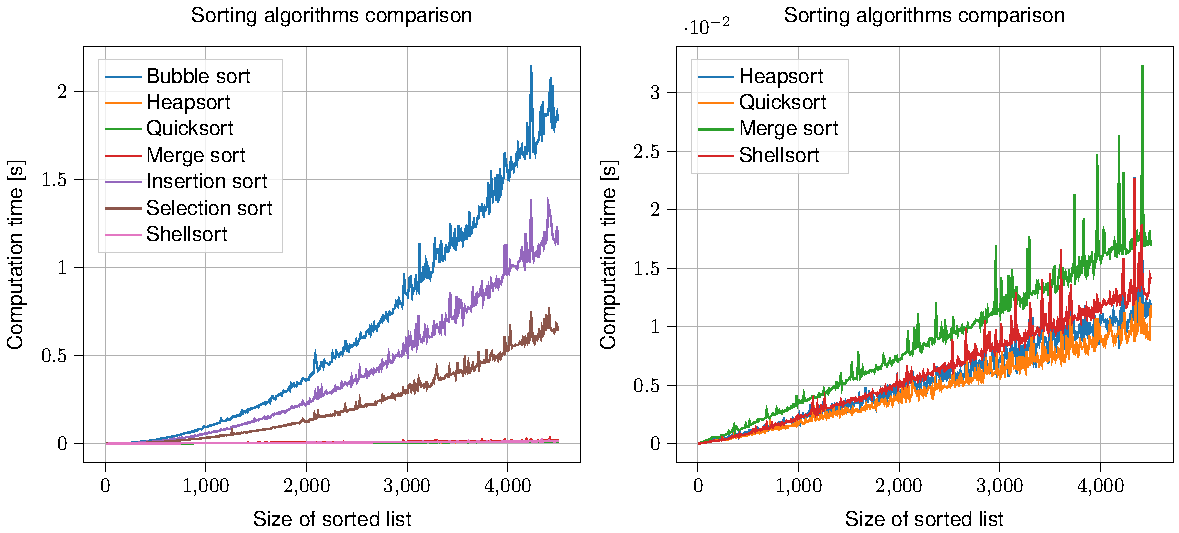
\includegraphics[scale = 0.75]{Sorting_algorithms_comparison}
\caption{Comparison of runtimes of sorting algorithms.}
\end{figure}
%\includefigurestatic[This is a caption.][scale = 0.35][h]{sorting-quadratic}

%\includefigurestatic[][scale = 0.35][h]{sorting-linear}

%\includefigurestatic[][scale = 0.35][h]{bubble-sort-complexity-2}


These can be verified experimentally  as seen in the following plot.  The random case grows quadratically just as the worst case does.  

\includefigurestatic[][scale = 0.35][h]{bubble-sort-computational-example}




There are some other relations that hold:
\begin{theorem}{Summations}{}
\begin{itemize}
\item $
\sum_{i=1}^{n} i = \frac{n(n+1)}{2}.
$
\item $
\sum_{i=1}^{n} i^2 = \frac{n(n+1)(2n+1)}{6}.
$
\item $
\sum_{i=1}^{n} i^3 = \frac{n^2(n+1)^2}{4}.
$
\end{itemize}
There are other formulas, but they get more complicated.  In general, we know that 
\begin{itemize}
\item $\sum_{i=1}^n i^k = O(n^{k+1}).$
\end{itemize}
\end{theorem}



\section{Problem, instance, size}
\subsection{Problem, instance}
\begin{definition}{Problem}{problem}
Is a {\bf generic} question/task that needs to be answered/solved. 

A problem is a ``collection of instances'' (see below).
\end{definition}


A  particular realization of a problem is defined next.

\begin{definition}{Instance}{instance}
An \emph{instance} is a specific case of a problem.  For example, for the problem of sorting, an instance we saw already is $(4,9,10,15,22,35)$.
\end{definition}

\subsection{Format and examples of problems/instances}

A problem is an abstract concept. We will write problems in the following format:
\begin{itemize}
	\item {\bf INPUT:} Generic data/instance.
	\item {\bf OUTPUT:} Question to be answered and/or task to be performed with the data.
\end{itemize}


{\bf Examples of problems/instances:}
	\begin{itemize}
	  \item Typical problems: optimization problems, decision problems, feasibility problems.
		\item LP and IP feasibility, TSP, IP minimization, Maximum cardinality independent set.
	\end{itemize}
	
	\subsection{Size of an instance}
	
The size of an instance is the {\em amount of information} required to represent the instance (in the computer).	Typically, this information is bounded by the quantity of numbers in the problem and the size of the numbers.

\begin{example}{Size of Sorting Problem}{}
Most of the time, we will think of the size of the sorting problem as 
$$
n,
$$
which is the number of numbers taht we need to sort.

However, we should also keep in mind that the size of the numbers is also important.  That is, if the numbers we are asked to sort take up 1 gigabyte of space to write down, then meerly comparing these numbers could take a long time. 

So to be more precise, the size of the problem is
$$
\# \text{ of bits to encode the problem }
$$
which can be upper bounded by 
$$
n \phi_{\max}
$$
where $\phi_{\max}$ is the maximum encoding size of a number given in the data.

For the sake of simplicity, we will typically ignore the size $\phi_{\max}$ in our complexity discussion.  A more rigirous discussion of complexity will be given in later (advanced) parts of the book.
\end{example}


\begin{example}{Size of Matching Problem}{}
The matching problem is presented as a graph $G= (V,E)$ and a set of costs $c_e$ for all $e \in E$.  Thus, the size of the problem can be deceibed as $|V| + |E|$, that is, in terms of the number of nodes and the number of edges in the graph.

\end{example}


\section{Complexity Classes}
In this subsection we will discuss the complexity classes P, NP, NP-Complete, and NP-Hard.  These classes help measure how difficult a problem is.  \textbf{Informally,} these classes can be thought of as 
\begin{itemize}
\item P - the class of efficiently solvable problems
\item NP - the class of efficiently checkable problems
\item NP-Hard - the class of problems that can solve any problem in NP
\item NP-Complete - the class of problems that are in both NP and are NP-Hard.
\end{itemize}
It is not known if $P$ is the same as NP, but it is conjectured that these are very different classes.  This would mean that the NP-Hard problems (and NP-Complete problems) are necessarily much more difficult than the problems in P.  See \refincludefigurestatic[Complexity class possibilities.  Most academics agree that the case $P \neq NP$ is more likely.]{wiki/File/complexity-classes.png}.

We will now discuss these classes more formally.
\subsection{P}
\begin{definition}{P}{}
P is the class of polynomially solvable problems.  P contains all problems for which there exists an algorithm that solves the problem in a run time bounded by a polynomial of input size. That is, $O(n^c)$ for some constant $c$.
\end{definition}

\begin{example}{Sorting}{}
The sorting problem can be solved in $O(n^2)$ time.  Thus, this problem is in $P$
\end{example}

\begin{example}{Complexity Minimum Spanning Tree}{}
The minimum size spanning tree problem is in P.  It can be solved, for instance, by Prim's algorithm, which  by runs in time $O(m \log n)$, where $m$ is the number of edges in the graph and $n$ is the number of nodes in the graph.  
\end{example}
\begin{example}{Complexity Linear Programming}{}
Linear programming is in P.  It can be solved by interior point methods in $O(n^{3.5} \phi)$ where $\phi$ represents the number of binary bits that are required to encode the problem.  These bits describe the matrix $A$, and vectors $c$ and $b$ that define the linear program.
\end{example}
\subsection{NP}
In this section, we will be more specific about the types of problems we want to consider.   In particular, we will consider \emph{decisions problems}.  These are problems where we only request an answer of "yes" or "no".

We can rephrase maximization problems as problems that ask "does there exists a solution with objective value greater than some number?"
\begin{example}{Maximum Matching as a decisions problem}{}
\textbf{Input:} A graph $G = (V,E)$ with weights $w_e$ for $e \in E$ and an objective goal $W$.

\begin{center}
\emph{
Does there exists a matching with objective value greater than $W$?}
\end{center}

\textbf{Output:} Either "yes" or "no".
\end{example}

%\begin{definition}{NP}{}
%\emph{NP} is the class of nondeterministic polynomial problems.  NP contains all problems in which membership can be verified in polynomial time from a \emph{certificate}.
%\end{definition}

We can now define the class of $\NP$.  
	
\begin{definition}{The class $\NP$}{NP2}
Is the set of all decision problems for which a YES answer for a  
particular instance can be {\bf verified} in polytime when provided a \emph{certificate}.

A certificate can be any additional information to help convince someone of a solution.  This should be describable in a compact way (polynomial in the size of the data).  Typically the certificate is simply a feasible solution.
\end{definition}
	
	{\bf Examples:}

\begin{multicols}{2}
\begin{itemize}
\item All problems in $\PP$
\item Integer programming
\item TSP
\item Binary knapsack
\item Maximum independent set
\item Subset sum
\item Partition
\item SAT, $k$-SAT
\item Clique
\end{itemize}
\end{multicols}


Thus, to show that a problem is in NP, you must do the following:
\begin{enumerate}
\item Describe a format for a certificate to the problem.
\item Show that given such a certificate, it is easy to verify the solution to the problem.
\end{enumerate}
\begin{example}{}{}
Integer Linear Programming is in NP.  More explicitly, the feasibility question of
\begin{center}
"Does there exists an integer vector $x$ that satisfies $Ax\leq b$"
\end{center}
is in NP.  

Although it turns out to be difficult to find such an $x$ or even prove that one exists, this problem is in NP for the following reason:  if you are given a particular $x$ and someone claims to you that it is a feasible solution to the problem, then you can easily check if they are correct.  
In this case, the vector $x$ that you were given is called a \emph{certificate}.

Note that it is easy to verify if $x$ is a solution to the problem because you just have to 
\begin{enumerate}
\item Check if $x$ is integer.
\item Use matrix multiplication to check if $Ax \leq b$ holds.
\end{enumerate}
\end{example}
\subsection{Problem Reductions}

We can compare different types of problems by showing that we can use one to solve the other.

A simple example of this is the problem \emph{Integer Programming} and the \emph{Matching Problem}.

Since we can model the \emph{Matching Problem} as an \emph{Integer Program}, then we know that we can solve the \emph{Matching Problem} provided that we can solve \emph{Integer Programs.}
\begin{center}
Matching Problem $\leq$ Integer Programming.
\end{center}

\begin{definition}{Reduction}{}
Given two problems $\mathcal A, \mathcal B$, we say $\mathcal A$ is \emph{reduced to} $\mathcal B$ (and we write $\mathcal A \leq \mathcal B$ when we can assert that if we can solve $\mathcal B$ in polynomial time, then we can also solve $\mathcal A$ in polynomial time.
\end{definition}

\subsection{NP-Hard}
The class of problems that are called \emph{NP-Hard} are those that can be used to solve any other problem in the NP class.  
That is, problem A is NP-Hard provided that for any problem B in NP there is a transformation of problem B that preserves the size of the problem, up to a polynomial factor, into a new problem that problem A can be used to solve.

Here we think of ``if problem A could be solved efficiently, then all problems in NP could be solved efficiently".

More specifically, we assume that we have an oracle for problem A that runs in polynomial time.  An oracle is an algorithm that for the problem that returns the solution of the problem in a time polynomial in the input.   This oracle can be thought of as a magic computer that gives us the answer to the problem.   
Thus, we say that problem A is NP-Complete provided that given an oracle for problem A, one can solve any other problem B in NP in polynomial time.

Note:  These problems are not necessarily in NP.

\subsection{NP-Complete}
The class of problems that are call \emph{NP-Complete} are those which are in NP and also NP-Hard.  

We know of many problems that are NP-Complete.  For example, binary integer programming feasibility is NP-Complete.  One can show that another problem is NP-complete by 
\begin{enumerate}
\item showing that it can be used to solve binary integer programming feasibility,
\item showing that the problem is in NP.
\end{enumerate}

The first problem proven to be NP-Complete is called \emph{3-SAT}~\cite{}.  3-SAT is a special case of the \emph{satisfiability problem}.   In a satisfiability problem, we have variables $X_1, \dots, X_n$ and we want to assign them values as either \true or \false.  The problem is described with \emph{AND} operations, denoted as $\land$,  with \emph{OR} operations, denoted as $\lor$, and with \emph{NOT} operations, denoted as $\neg$.  The \emph{AND} operation $X_1 \land X_2$ returns $\true$ if BOTH $X_1$ and $X_2$ are true.  The \emph{OR} operation $X_1 \lor X_2$ returns $\true$ if AT LEAST ONE OF  $X_1$ and $X_2$ are true.  Lastly, the \emph{NOT} operation $\neg X_1$ returns there opposite of the value of $X_1$.

These can be described in the following table
\begin{align}
\true \land \true = \true\\
\true \land \false = \false\\
\false \land \false = \false\\
\false \land \true = \false
\end{align}

\begin{align}
\true \lor \true = \true\\
\true \lor \false = \true\\
\false \lor \false = \false\\
\false \lor \true = \true
\end{align}

\begin{align}
\neg \true = \false\\
\neg \false = \true
\end{align}

For example, \textbf{Missing code here}
%$$
%\neg \true \lor \false \lor \true = \true \ \ \ \ \true \and \neg \true = \false
%$$
A \emph{logical expression} is a sequence of logical operations on variables $X_1, \dots, X_n$, such that 
\begin{equation}
(X_1 \land \neg X_2 \lor X_3) \land (X_1 \lor \neg X_3) \lor (X_1 \land X_2 \land X_3).
\end{equation}

A \emph{clause} is a logical expression that only contains the operations $\lor$ and $\neg$ and is not nested (with parentheses), such as 
\begin{equation}
X_1 \lor \neg X_2 \lor X_3 \lor \neg X_4.
\end{equation}

A fundamental result about logical expressions is that they can always be reduced to a sequence of clauses that are joined by $\land$ operations, such as 
\begin{equation}
(X_1 \lor \neg X_2 \lor X_3 \lor \neg X_4) \land (X_1 \lor X_2 \lor X_3) \land (X_2 \lor \neg X_3 \lor \neg X_4 \lor X_5).
\end{equation}
The satisfiability problem takes as input a logical expression in this format and asks if there is an assignment of \true  or \false to each variable $X_i$ that makes the expression \true.  The 3-SAT problem is a special case where the clauses have only three variables in them.
 
\begin{general}{3-SAT}{\npcomplete}
Given a logical expression in $n$ variables where each clause has only 3 variables, decide if there is an assignment to the variables that makes the expression \true.
\end{general}


\begin{general}{Binary Integer Programming}{\npcomplete}
Binary Integer Programming can easily be shown to be in NP, since verifying solutions to BIP can be done by checking a linear system of inequalities.  

Furthermore, it can be shown to be NP-Complete since it can be used to solve 3-SAT.  That is, given an oracle for BIP, since 3-SAT can be modeled as a BIP,  the 3-SAT could be solved in oracle-polynomial time.
\end{general}

\section{Problems and Algorithms}
We will discuss the following concepts:
\begin{itemize}
\item Feasible solutions
\item Optimal solutions
\item Approximate solutions
\item Heuristics
\item Exact Algorithms
\item Approximation Algorithms
\item Complexity class relations
\end{itemize}


\subsection{Matching Problem}




\begin{definition}{Matching}{}
Given a graph $G = (V,E)$, a \emph{matching} is a subset $E' \subseteq E$ such that no vertex $v \in V$ is contained in more than one edge in $E'$.  \\
A \emph{perfect matching} is a matching were every vertex is connected to an edges in $E'$.\\
A \emph{maximal matching} is a matching $E'$ such that there is no matching $E''$ that strictly contains it.
\end{definition}


\begin{figure}[H]
\todo[inline]{
INCLUDE PICTURES OF MATCHINGS
%\includegraphics[scale = 0.5]{matchings}\footnotemark
}
\label{fig:matching}
\caption{Two possible matchings.  On the left, we have a perfect matchings (all nodes are matched).  On the right, a feasible matching, but not a perfect matching since not all nodes are matched.}

\end{figure}







\begin{definition}{Maximum Weight Matching}{}
Given a graph $G = (V,E)$, with associated weights $w_e\geq 0$ for all $e \in E$, a \emph{maximum weight matching} is a matching that maximizes the sum of the weights in the matching.
\end{definition}


\includefigurestatic[][scale = 0.5][h]{graph-for-matching-maximal}





%
%\begin{enumerate}
%\item Feasible solution
%\item Greedy Procedure
%\end{enumerate}
%
%\begin{enumerate}
%\item Procedure
%\item Algorithm
%\begin{enumerate}
%\item Heuristic
%\item Approximation
%\item Exact
%\end{enumerate}
%\end{enumerate}
\subsubsection{Greedy Algorithm for Maximal Matching}
The greedy algorithm iteratively adds the edge with largest weight that is feasible to add.  
\begin{general}{Greedy Algorithm for Maximal Matching}{Complexity: $O(|E|\log(|V|))$}
\label{alg:greedy-matching}
\begin{enumerate}
\item Begin with an empty graph $(M = \emptyset)$
\item Label the edges in the graph such that $w(e_1) \geq w(e_2) \geq \dots \geq w(e_m)$
\item For $i=1, \dots, m$\\
\indent  If $M \cup\{e_i\}$ is a valid matching (i.e., no vertex is incident with two edges), then set $M \leftarrow M \cup \{e_i\}$ (i.e., add edge $e_i$ to the graph $M$)
\item Return $M$
\end{enumerate}
\end{general}

\begin{theorem}{Greedy algorithm gives a 2-approximation [\cite{Avis83}]}{}
The greedy algorithm finds a 2-approximation of the maximum weighted matching problem.  That is, $w(M_{greedy}) \geq \tfrac{1}{2} w(M^*)$.
\end{theorem}
%\begin{proof}
%Proof. Let x be the weight of the first edge ( i , j ) that is selected by GREEDY, so that x is in fact an edge of maximum weight in G. Now when (i,j) and all incident edges are deleted, at most two edges of the optimal matching may be removed. Further,thesumoftheirweightscannotexceed2x. Theothern-2ormoreedgesof the optimal matching are candidates for selection at the next iteration of GREEDY. The argument may be repeated for each of the first fniterations of GREEDYII. Since all edge weights are non-negative, the theorem is proved.
%\end{proof}


\subsubsection{Other algorithms to look at}
\begin{enumerate}
\item Improved  Algorithm \cite{DRAKE2003211}
\item Blossom Algorithm \href{https://en.wikipedia.org/wiki/Blossom_algorithm}{Wikipedia}
\end{enumerate}



\subsection{Minimum Spanning Tree}
\begin{definition}{Spanning Tree}{}
Given a graph $G = (V,E)$, a \emph{spanning tree} connected, acyclic subgraph $T$ that contains every node in $V$.
\end{definition}

\includefigurestatic[][scale = 0.=5][h]{spanning-tree}

\begin{definition}{Max weight spanning tree}{}
Given a graph $G = (V,E)$, with associated weights $w_e\geq 0$ for all $e \in E$, a \emph{maximum weight spanning tree} is a spanning tree maximizes the sum of the edge weights.
\end{definition}


\includefigurestatic[][scale = 0.5][h]{spanning-tree-MST}


\begin{lemma}{Edges and Spanning Trees}{}
Let  $G$ be a  connected graph with $n$ vertices.  
\begin{enumerate}
\item $T$ is a spanning tree of $G$ if and only if $T$ has $n-1$ edges and is connected.
\item Any subgraph $S$ of $G$ with more than $n-1$ edges contains a cycle.
\end{enumerate}
\end{lemma}


See Section~\ref{sec:spanning-tree-models} for integer programming formulations of this problem.  
\subsection{Kruskal's algorithm}
\begin{general}{Kruskal  - for Minimum Spanning tree}{Complexity: $O(|E| \log(|V|)$}
\label{alg:Kruskal}
\begin{enumerate}
\item Begin with an empty tree $(T = \emptyset)$
\item Label the edges in the graph such that $w(e_1) \leq w(e_2) \leq \dots \leq w(e_m)$
\item For $i=1, \dots, m$\\
\indent  If $T \cup\{e_i\}$ is acyclic, then set $T \leftarrow T \cup \{e_i\}$
\item Return $T$
\end{enumerate}
\end{general}


%\begin{general}{Acyclic Graph}{}
%\label{alg:Acyclic}
%\textbf{Input:} An acyclic graph $T$ and an edge $e$
%\textbf{Output:} Either "Yes" - $T \cup \{e\}$ contains a cycle or "No" it does not contain a cycle.
%\begin{enumerate}
%\item Begin with an empty tree $(T = \emptyset)$
%\item Label the edges in the graph such that $w(e_1) \leq w(e_2) \leq \dots \leq w(e_m)$
%\item For $i=1, \dots, m$\\
%\indent  If $T \cup\{e_i\}$ is acyclic, then set $T \leftarrow T \cup \{e_i\}$
%\item Return $T$
%\end{enumerate}
%\end{general}


%\begin{proof}
%
%\end{proof}

\subsubsection{Prim's Algorithm}


\subsection{Traveling Salesman Problem}

See Section~\ref{sec:tsp-models} for integer programming formulations of this problem.  Also, hill climbing algorithms for this problem such as 2-Opt, simulated annealing, and tabu search will be discussed in Section~\ref{sec:IP-Heuristics}.

\subsubsection{Nearest Neighbor - Construction Heuristic}

We will discuss heuristics more later in this book.   For now, present this construction heuristic as a simple algorithmic example.   


Starting from any node, add the edge to the next closest node.  Continue this process.
\begin{general}{Nearest Neighbor}{Complexity: $O(n^2)$}
\label{heuristic:nearestNeighbor}
\begin{enumerate}
\item Start from any node (lets call this node 1) and label this as your current node.
\item Pick the next current node as the one that is closest to the current node that has not yet been visited.
\item Repeat step 2 until all nodes are in the tour.
\end{enumerate}
\end{general}

\subsubsection{Double Spanning Tree - 2-Apx}
We can use a minimum spanning tree algorithm to find a provably okay solution to the TSP, provided certain properties of the graph are satisfied.  

Graphs with nice properties are often easier to handle and typically graphs found in the real world have some nice properties. The \emph{triangle inequality} comes from the idea of a triangle that the sum of the lengths of two sides always are longer than the length of the third side. See \refincludefigurestatic{wiki/File/triangle_inequality.png}


\begin{definition}{Triangle Inequality on a Graph}{}
A complete, weighted graph $G$ (i.e., a graph that has all possible edges and a weight assigned to each edge) satisfies the \emph{triangle inequality} provided that for ever triple of vertices $a,b,c$ and edges $e_{ab}, e_{bc}, e_{ac}$, we have that 
\[
w(e_{ab}) + w(e_{bc}) \geq w(e_{ac}).
\]
\end{definition}



\begin{algorithm}
\algorithmicrequire{A graph $G = (V,E)$ that satisfies the triangle inequality}\\
\algorithmicensure{A tour that is a 2-Apx of the optimal solution}
\caption{Double Spanning Tree}\label{alg:double-spanning-tree}
\begin{algorithmic}[1]
	\State Compute a minimum spanning tree $T$ of $G$.
 	\State Double each edge in the minimum spanning tree (i.e., if edge $e_{ab}$ is in $T$, add edge $e_{ba}$. 
	\State Compute an Eulerian Tour  using these edges.
	\State Return tour that visits vertices in the order the Eulerian Tour visits them, but without repeating any vertices.
	\end{algorithmic}
\end{algorithm}

Let $S$ be the resulting tour and let $S^*$ be an optimal tour.
Since the resulting tour is feasible, it will satisfy 
\[
w(S^*) \leq w(S).
\]
But we also know that the weight of a minimum spanning tree $T$ is less than that of the optimal tour, hence
\[
w(T) \leq w(S^*).
\]
Lastly, due to the triangle inequality we know that 
\[
w(S) \leq 2 w(T),
\]
since replacing any edge in the Eulerian tour with a more direct edge only reduces the total weight.

Putting this together, we have

\[w(S) \leq 2w(T) \leq 2 w(S^*)\]
and hence, $S$ is a 2-approximation of the optimal solution.


\subsubsection{Christofides - Approximation Algorithm - $(3/2)$-Apx}
If we combine algorithms for minimum spanning tree and matching, we can find a better approximation algorithm.  This is given by Christofides.  Again, this is in the case where the graph satisfies the triangle inequality.  See 
\href{https://en.wikipedia.org/wiki/Christofides_algorithm}{Wikipedia - Christofides Algorithm} or \href{https://resources.mpi-inf.mpg.de/conferences/adfocs-15/material/Ola-Lect1.pdf}{Ola Svensson Lecture Slides} for more detail.


\section{Resources}
\begin{resource}
\begin{itemize}
\item \href{http://web.mit.edu/16.070/www/lecture/big_o.pdf}{MIT Lecture Notes - Big O}
\item \href{https://www.youtube.com/watch?v=YX40hbAHx3s}{Youtube! - P versus NP}
\end{itemize}
\end{resource}

\begin{resource}
Bubble Sort
\begin{itemize}
\item \href{https://en.wikipedia.org/wiki/Bubble_sort}{Wikipedia}
\end{itemize}
\end{resource}
\begin{resource}
Kruskal
\href{https://en.wikipedia.org/wiki/Kruskal\%27s_algorithm}{Wikipedia}
\end{resource}
\begin{resource}
Prim's Algorithm
\begin{itemize}
\item \href{https://en.wikipedia.org/wiki/Prim\%27s_algorithm}{Wikipedia}
\item \href{http://www.texample.net/tikz/examples/prims-algorithm/}{TeXAmple - Figure for min spannig tree}
\end{itemize}
\end{resource}
\begin{resource}
Nearest Neighbor for TSP
\href{https://en.wikipedia.org/wiki/Nearest_neighbour_algorithm}{Wikipedia}
\end{resource}

\subsection{Advanced - NP Completeness Reductions}
\textbf{Problem: Subset Sum}

Instance: A set of $n$ positive integers $S$ and a target positive integer $t$.

Question: Is there a subset of $S$ that adds up to $t$?

\textbf{Reduction:} We'll reduce the problem "3SAT" to "Subset Sum".

Given an instance of 3SAT with $m$ clauses and $n$ variables, we'll create a corresponding instance of Subset Sum as follows:

For each variable, create two positive integers: $2^{(i-1)}$ and $2^{i}$, where $i$ is the index of the variable.

For each clause $(x$ or $y$ or $z)$, create a target integer $t$ equal to $2^{(m+n)} + 2^{(x-1)} + 2^{(y-1)} + 2^{(z-1)}$, where $x, y, z$ are the indices of the variables in the clause.

The set $S$ for Subset Sum will be the $n$ positive integers created for the $n$ variables, plus all the target integers created for the $m$ clauses.

\textbf{Claim:} The 3SAT instance is satisfiable if and only if the corresponding Subset Sum instance has a solution.

\textbf{Proof:}

If the 3SAT instance is satisfiable, then for each clause $(x$ or $y$ or $z)$, at least one of the variables $x, y,$ or $z$ must be set to true. Thus, we can include the corresponding positive integers in our solution for the Subset Sum instance, and the solution will sum up to the target $t$ for that clause.

If the Subset Sum instance has a solution, then for each clause $t$, there must be a subset of $S$ that sums up to $t$. We can set the variables corresponding to the positive integers included in the subset to true, and set all other variables to false. This will result in a satisfying assignment for the 3SAT instance.

Since 3SAT is NP-complete, and we have shown that Subset Sum can be reduced to 3SAT in polynomial time, it follows that Subset Sum is also NP-complete.
%\end{document}